The tests presented in this section are tests of discrete events, not of 
simulated or propagated values.  The output from each test is found in the 
appropriate run directory's \textit{mass.out} file.  
This document presents the analytic solution for each of the testing 
scenarios.  The analytic solution can be compared against the data output. 
Since there were no 
discrepancies to analyze, those output data have not been duplicated in this 
document, but are available for the reader to independently verify the claims 
made herein.

\subsection{Attachment Tests}
\test{Two-Object Combination}\label{test:mass_01}
\begin{description}
\item[Purpose:] \ \newline
The purpose of this test is to examine the ability to calculate the composite 
properties of two adjoined objects.
In this test, the MassBody objects are two identical
right rectangular prisms.\\
SIM directory: models/dynamics/body\_action/verif/SIM\_verif\_attach\_mass\\
Run directory: RUN\_01 RUN\_101
\item[Requirements:] \ \newline
Successful completion of this test partially satisfies
requirements~\traceref{reqt:CoM_location}, \traceref{reqt:composite_mass}, 
\traceref{reqt:composite_inertia}, and \traceref{reqt:attach}.
\item[Procedure:]\ \newline
In these test, the two objects were conceptualized with uniform density and 
dimensions $(1.0, ~1.0, ~2.0) ~m$.  The strucural-axes and body-axes were 
defined to be equivalent, the mass set to $1.0 kg$, and the inertia tensor 
specified 
as:
\begin{equation*}
\begin{bmatrix} \frac{5}{12} & 0 & 0 \\ 0 & \frac{5}{12} & 0 \\ 0 & 0 & 
\frac{1}{6} \end{bmatrix} kg ~ m^2 
\end{equation*}
(thereby defining the body-axes along the principal axes, and placing the $2.0 
~m$ length on the z-axis).

Although the two objects are identical, it is necessary to denote one the 
\textit{parent} and one the \textit{child}.  The \textit{child} will be 
attached to the \textit{parent}.

In the first test, the attachment of child to parent was performed by the 
offset-orientation method.  
The child was attached with an offset of $1.5 ~m$ and a 
relative orientation represented as a rotation of 90 degrees about the parent 
x-axis.

In the second test, the attachment of child to parent was performed by the 
mass-point method. A mass point was defined on the child body with position 
$(0.0, ~0.0,~1.0) m$ 
and an orientation (with respect to the child structural axes) expressed with 
the transformation matrix: 
\begin{equation*}
\begin{bmatrix} 0 & 0 & 1 \\ 0 & -1 & 0 \\ 1 & 0 & 0 \end{bmatrix}
\end{equation*}
The parent body defines a mass point with position  $(0.0, ~0.5, ~0.0) m$ and 
an orientation expressed with the transformation matrix 
\begin{equation*}
 \begin{bmatrix} 0 & 1 
& 0 \\ 0 & 0 & 1 \\ 1 & 0 & 0 \end{bmatrix}
\end{equation*}

In both tests, the resulting attachment should be as illustrated in 
Figure~\ref{two_rect}, with the parent body beneath the child body.  
The parent structural axes have origin at the center of the parent body, and 
are oriented as follows:
\begin{itemize}
 \item x-axis into the page
 \item y-axis bottom-to-top
 \item z-axis left-to-right
\end{itemize}
.

The computed positions and composite inertia tensors were then compared 
against separate analytical computations.

\begin{figure}[h]
\begin{center}
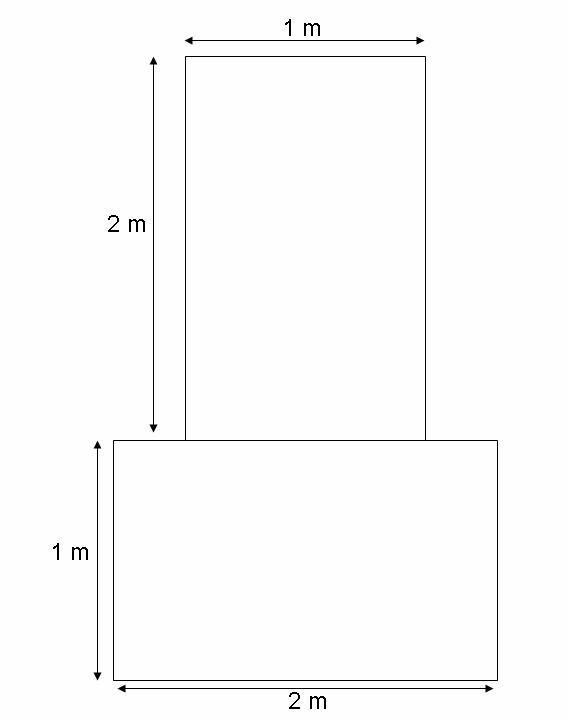
\includegraphics[height=80mm]{pics/two_rect.jpg} 
\caption{Diagram of composite Mass-body for Test 1}
\label{two_rect}
\end{center}
\end{figure}


\item[Results:]\ \newline
The inertia for each individual body in Figure~\ref{two_rect} is calculated 
using standard equations for a uniform density body (see, 
for example, Bedford~\cite{Bedford}) and verified against the input values.

For the composite-body, in both tests, the position of the center of mass 
agrees with the analytical result of $(0.0,~0.75,~0.0) m$.  The composite-body 
inertia tensors also agree with the analytical result of $\begin{bmatrix} 
\frac{47}{24} & 0 & 0 \\ 0 & \frac{7}{12} & 0 \\ 0 & 0 & \frac{41}{24} 
\end{bmatrix} kg ~ m^2$

\end{description}

\clearpage






\test{Complex Tree, Three-object Combinations}\label{test:mass_02}
\begin{description}
\item[Purpose:] \ \newline
We have already demonstrated that two objects can be attached (in 
Test~\ref{test:mass_01}).  The purpose of this test is to investigate more 
complex tree structure by attaching three objects together.  Two different 
configurations, one in which a parent has two children attached, and one in 
which a parent has a child, which has an additional child attached to it, are 
used.  These configurations verify the ability to handle multiple children, 
and multi-generational trees.
\newline
SIM directory: models/dynamics/body\_action/verif/SIM\_verif\_attach\_mass\\
Run directory: RUN\_02 RUN\_03 RUN\_04  RUN\_102 RUN\_103 RUN\_104
\item[Requirements:] \ \newline
Successful completion of this test partially satisfies
requirements \traceref{reqt:CoM_location}, \traceref{reqt:composite_mass}, 
\traceref{reqt:composite_inertia}, and \traceref{reqt:attach}.
\item[Procedure:]\ \newline
Three identical objects, equivalent to those used in 
test~\ref{test:mass_01} were stacked along each of the three axes.  As with 
test~\ref{test:mass_01}, both the position-orientation and mass-point 
specifications were tested.  The setup of the tests is as follows:
\begin{itemize}
 \item RUN\_02 Stacked on y-axis using the position-orientation specification.
 Parent 
 has 2 children with identical orientations, located at $(0,~\pm1.0,~0.0) m$
 \item RUN\_03 Stacked on x-axis, using the position-orientation 
 specification.  Parent 
 has 1 child (Child1) with identical orientation to Parent, and relative 
 position at $(1.0,~0.0,~0.0)~m$.
 Child1 has 1 child (Child2), with identical orientation to Child1 (so also 
 identical orientation to Parent), and relative position at 
 $(1.0,~0.0,~0.0)~m$ (so Child2 is at $(2.0,~0.0,~0.0)~m$ relative to Parent).
 \item RUN\_04 Stacked on z-axis, using the position-orientation 
 specification. Parent 
 has 1 child (Child1) with identical orientation to Parent and relative 
 position at $(0.0,~0.0,~-2.0)~m$.  
 Child1 has 1 child, also with identical orientation and relative position at 
 $(0.0,~0.0,-2.0)~m$.
 \item RUN\_102 Stacked on y-axis, using the mass-point specification.  
 Parent has 2 
 children and 2 mass-points located at the center of its $\pm y-$faces.  The 
 two children both have mass points on their respective $y-$faces.  The 
 orientations of all four mass points have a $\pm 90^o$ yaw (such that each 
 matching pair has one point with a positive yaw and one with a negative yaw).
 \item RUN\_103 Stacked on x-axis, using the mass-point specification.
 The parent has
 one mass point, at the center of its $+x-$face and oriented with the body 
 that is used to attach to the first child.  The first child has two mass 
 points, one at the center of its $-x-$face with a $180^o$ yaw that is used 
 to attach it to the parent, and one at the center of its $+x-$face and 
 oriented with the body that is used to attach it to the second child.  The 
 second child has one mass point at its $-x-$face with a $180^o$ yaw that is 
 used to attach it to the first child.
 \item RUN\_104 Stacked on z-axis, using the mass-point specification. 
 The parent has 
 one mass point, at the center of its $-z-$face and oriented with a 
 transformation matrix $\begin{bmatrix} 0 & 0 & -1 \\ 0 & 1 & 0 \\ 1 & 0 & 0 
 \end{bmatrix}$ that is used to attach to the first child.  The first child 
 has two mass points, one at the center of its $+z-$face with a transformation 
 matrix $\begin{bmatrix} 0 & 0 & 1 \\ 0 & -1 & 0 \\ 1 & 0 & 0 \end{bmatrix}$ 
 that is used to attach it to the parent, and one at the center of its 
 $-z-$face with a transformation matrix $\begin{bmatrix} 0 & 0 & -1 \\ 0 & 1 & 
 0 \\ 1 & 0 & 0 \end{bmatrix}$ that is used to attach it to the second child.  
 The second child has one mass point at its $+z-$face with a with a 
 transformation matrix $\begin{bmatrix} 0 & 0 & 1 \\ 0 & -1 & 0 \\ 1 & 0 & 0 
 \end{bmatrix}$ that is used to attach it to the first child.
\end{itemize}

In all 6 runs, the resulting orientation of all three bodies is identical.  In 
runs 02 and 102, the parent provides the central body with the children 
attached symmetrically, one on each side.  In the other 4 runs, the parent is 
located at one end of the stack.

Figure \ref{3_stack_z} illustrates the configuration for runs 04 and 104, with 
the parent to the right, the first child in the center, and the second child 
at the left.  The configurations for the other runs are similarly simple, 
except on other axes.


\begin{figure}[h]
\begin{center}
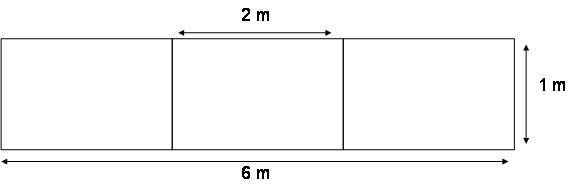
\includegraphics[height=40mm]{pics/stack_z.jpg}
\caption{Diagram of stacked body for test}
\label{3_stack_z}
\end{center}
\end{figure}

\item[Results:]\ \newline
For all six runs, the mass of the composite body agrees with the predicted $3~ 
kg$.

The position of the center of mass should be as follows:
\begin{itemize}
 \item Runs 02 and 102:  $(0.0,~0.0,~0.0)$ (parent is at the center)
 \item Runs 03 and 103:  $(1.0,~0.0,~0.0)$ (parent is at one end)
 \item Runs 04 and 104:  $(0.0,~0.0,-2.0)$ (parent is at one end)
\end{itemize}

The moments of inertia should be:
\begin{itemize}
 \item Runs 02 and 102:  $3\begin{bmatrix} \frac{5}{12} & 0 & 0 \\ 0 & 
 \frac{5}{12} & 0 \\ 0 & 0 & \frac{1}{6} \end{bmatrix} kg ~ m^2 + 
 2\begin{bmatrix} 1 & 0 & 0 \\ 0 & 0 & 0 \\ 0 & 0 & 1 \end{bmatrix}kg ~ m^2  = 
 \begin{bmatrix} \frac{13}{4} & 0 & 0 \\ 0 & \frac{5}{4} & 0 \\ 0 & 0 & 
 \frac{5}{2} \end{bmatrix}kg ~ m^2$
 \item Runs 03 and 103:  $\begin{bmatrix} \frac{5}{4} & 0 & 0 \\ 0 & 
 \frac{13}{4} & 0 \\ 0 & 0 & \frac{5}{2} \end{bmatrix}kg ~ m^2$ 
 \item Runs 04 and 104:  $\begin{bmatrix} \frac{37}{4} & 0 & 0 \\ 0 & 
 \frac{37}{4} & 0 \\ 0 & 0 & \frac{1}{2} \end{bmatrix}kg ~ m^2$ 
\end{itemize}


All results agreed with predictions.
\end{description}




\test{Compound, non-Root Attachment}\label{test:mass_08}
\begin{description}
\item[Purpose:] \ \newline
The purpose of this test is to confirm that the \ModelDesc correctly manages 
the mass-properties when a composite body is attached to a parent.  The test further verifies the legitimacy of commanding a non-root component of the mass tree to attach to the parent.

\item SIM directory: 
models/dynamics/body\_action/verif/SIM\_verif\_attach\_mass\\
Run directory: RUN\_08 RUN\_108

\item[Requirements:] \ \newline
Successful completion of this test completes the satisfaction of 
requirements \traceref{reqt:CoM_location}, \traceref{reqt:composite_mass}, 
\traceref{reqt:composite_inertia}, and~\traceref{reqt:attach}.

\item[Procedure:]\ \newline
This test utilizes four flat plates similar to those used in previous 
tests.  The four plates are attached to one another in the following sequence
\begin{enumerate}
 \item child2 is attached to child1
 \item child3 is attached to child2
 \item child3 is attached to parent. 
\end{enumerate}

Following the system established in previous tests, RUN\_08 has the attachment 
performed using offset-orientation specification, while RUN\_108 uses the 
mass-point specification to perform the same task.

Figure~\ref{fig:four_plates} illustrates the relative orientation and the 
physical connections between the four plates.

\begin{figure}[h]
\begin{center}
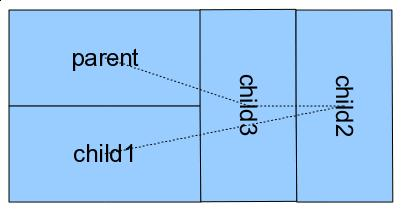
\includegraphics[height=40mm]{pics/four_plates.jpg}
\caption{Plate arrangement for test}
\label{fig:four_plates}
\end{center}
\end{figure}

Notice that child1 and child2 are not actually in contact.  This is entirely 
legitimate, although to perform the attachment using mass-points (in 
RUN\_108), at least one of the mass-points must be dislocated from the actual 
mass body (we arbitrarily chose to do this to child2).

In contrast, Figure~\ref{fig:four_plates_tree} illustrates the progression of 
the development of the mass trees as each attachment is performed.  Notice 
that in the mass-tree, \textit{child3} is not attached to \textit{parent}.  
In the mass tree, it is the root of the tree containing 
\textit{child3} that is attached to \textit{parent}.

\begin{figure}[h]
\begin{center}
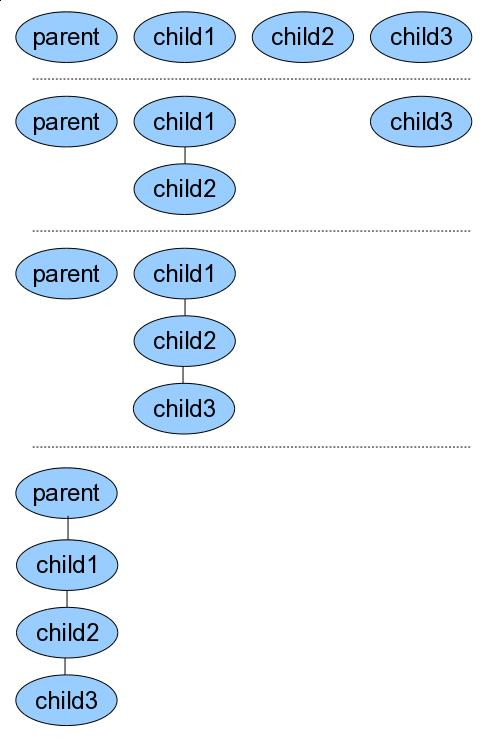
\includegraphics[height=120mm]{pics/four_plates_tree.jpg}
\caption[Mass Tree Evolution]
{Four frames (top to bottom) showing the sequential evolution of the 
mass tree as the objects are attached.}
\label{fig:four_plates_tree}
\end{center}
\end{figure}

\item[Results:]\ \newline
The resulting conter of mass location relative to the parent structure-point 
(center of the parent plate) is $(-0.5,~0.0,~1.0)~m$ (the point where plates 
\textit{parent}, \textit{child1} and \textit{child3} meet).
The inertia tensor should be that of a uniform rectangular plate of mass 
$4.0~kg$ and sides $(2.0,~0.0,~4.0)~m$.
\begin{equation*}
I_{comp,CM} = 
   \begin{bmatrix} \frac{16}{3} & 0.0   & 0.0  \\
                   0.0   & \frac{20}{3} & 0.0   \\
                    0.0  & 0.0   & \frac{4}{3} 
   \end{bmatrix}
\end{equation*} 

For Child1, the composite-body comprises the three plates \textit{child1}, 
\textit{child2}, and \textit{child3}, positioned with respect to the child1 
structure-point (and center of mass) at $(0,~0,~0)~m$, 
$(\frac{1}{2},~0,~\frac{3}{2})~m$, and $(\frac{1}{2},~0,~\frac{5}{2})~m$ 
respectively.  Thus, the center of mass of the composite body should be at 
$(\frac{1}{3},~0,\frac{4}{3})~m$.  When accumulating the inertia tensor, 
remember that \textit{child2} and \textit{child3} are oriented so that, 
oriented to the body-axes of \textit{child1}, their inertia tensors are 
\begin{equation*}
\begin{bmatrix} \frac{1}{12} & 0   & 0  \\
                   0  & \frac{5}{12} & 0   \\
                    0  & 0   & \frac{1}{3} 
   \end{bmatrix}
\end{equation*} 

The \textit{child1}-based composite body inertia tensor should then be
\begin{equation*}
\begin{split}
I_{child1-composite,body} & = 
    \begin{bmatrix} \frac{1}{3} & 0   & 0  \\
                   0  & \frac{5}{12} & 0   \\
                    0  & 0   & \frac{1}{12} 
   \end{bmatrix}
   +2
   \begin{bmatrix} \frac{1}{12} & 0   & 0  \\
                   0   & \frac{5}{12} & 0   \\
                    0  & 0   & \frac{1}{3} 
   \end{bmatrix}
   +\\
    & \ \ \ \ \ \ \ \ \ 
\begin{bmatrix} \frac{16}{9} & 0   & -\frac{4}{9}  \\
                   0   & \frac{17}{9} & 0   \\
                    -\frac{4}{9}  & 0   & \frac{1}{9} 
   \end{bmatrix}
  +
\begin{bmatrix} \frac{1}{36} & 0   & -\frac{1}{36}  \\
                   0   & \frac{2}{36} & 0   \\
                    -\frac{1}{36}  & 0   & \frac{1}{36} 
   \end{bmatrix}
   +
\begin{bmatrix} \frac{49}{36} & 0   & -\frac{7}{36}  \\
                   0   & \frac{50}{36} & 0   \\
                    -\frac{7}{36}  & 0   & \frac{1}{36} 
   \end{bmatrix}
    \\
   & =
   \begin{bmatrix} \frac{11}{3} & 0   & -\frac{2}{3}  \\
                   0   & \frac{55}{12} & 0   \\
                    -\frac{2}{3}  & 0   & \frac{11}{12} 
   \end{bmatrix}
\end{split}
\end{equation*} 

When considering the composite-body properties of \textit{child2}, notice that 
the body-axes have been rotated.  The composite-body now comprises 
\textit{child2} and \textit{child3}, which makes a square plate of side 
$2.0~m$ and mass $2.0~kg$, with center of mass at $(\frac{1}{2},~0,~0)~m$ from 
the structure-point of \textit{child2}.  The corresponding inertia tensor is, 
as we have seen in previous tests:
\begin{equation*}
\begin{bmatrix} \frac{2}{3} & 0   & 0  \\
                   0  & \frac{4}{3} & 0   \\
                    0  & 0   & \frac{2}{3} 
   \end{bmatrix}
\end{equation*} 

Finally, the composite-body properties of \textit{child3} should be the same 
as its core-properties, since it has no children.

All results match predictions.

\end{description}

\clearpage






\subsection{Detach Process}
\test{Detach One of Four Plates}\label{test:mass_10}
\begin{description}
\item[Purpose:] \ \newline
The purpose of this test is to confirm that the \ModelDesc
correctly monitors mass properties through a detach process.

SIM directory: models/dynamics/body\_action/verif/SIM\_verif\_attach\_mass\\
Run directory: RUN\_10 RUN\_110

\item[Requirements:] \ \newline
Successful completion of this test satisfies
requirement~\traceref{reqt:detach}.

\begin{figure}[h]
\begin{center}
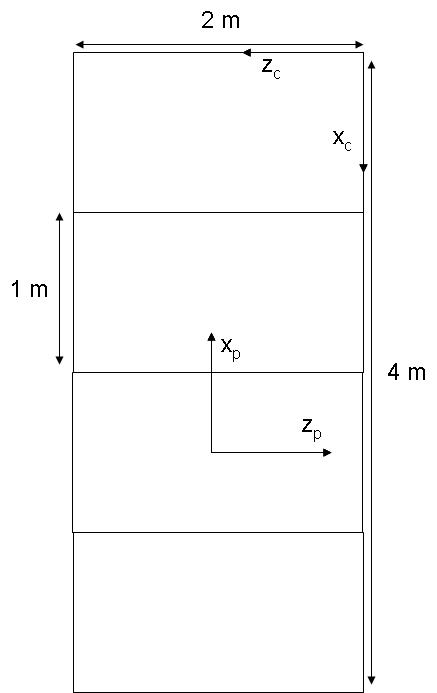
\includegraphics[height=80mm]{pics/4stack_x_rot.jpg}
\caption{Diagram of Test Setup and Reference Frames}
\label{fig:4body_axis_2}
\end{center}
\end{figure}

\item[Procedure:]\ \newline
In this test, we use four flat plates again, stacked along the x-axis as shown 
in Figure~\ref{fig:4body_axis_2}.  All four plates are attached directly as 
children of the parent, and appear in order of decreasing x (top to bottom):
\begin{enumerate}
 \item child2
 \item child3
 \item parent
 \item child1
\end{enumerate}

To add to the complexity, the inertia tensor of \textit{child2} is defined 
with respect to its structure-point, which is defined in one corner (the top 
right corner in Figure~\ref{fig:4body_axis_2}); the appropriate transformation 
of such a specification into the body-axes has already been verified in 
test~\ref{test:mass_05}, and the attach process verified in 
test~\ref{test:mass_07}.  It remains only to demonstrate that the mass 
properties are correct following detachment.

At some time after initialization, \textit{child2} is detached from the mass 
tree, leaving only three uniform plates attached together. These three plates 
can be represented as a single uniform plate, of dimensions $(3,~0,~2)~m$ and 
mass $3~kg$.  The parent structure-point, at the center of the parent plate, 
is now at the geometric center of the composite plate, so the composite body 
position should be $(0,~0,~0)~m$.

The composite-body inertia tensor should be that of a uniform plate:
\begin{equation*}
I_{parent-comp,body} = 
   \begin{bmatrix} 1 & 0   & 0  \\
                   0   & \frac{13}{4} & 0   \\
                    0  & 0   & \frac{9}{4} 
   \end{bmatrix}
\end{equation*} 

\textit{Child2} properties should remain those of the atomic body.

\item[Results:]\ \newline
The results are as expected.


\end{description}

\subsection{Reattach Process}
\test{Four Plates with Reattachment}\label{test:mass_11}
\begin{description}
\item[Purpose:] \ \newline
The purpose of this test is to confirm that the \ModelDesc
can move an attached body from one location to another (with respect to its 
parent).  It also further
confirms the mass model's capability to calculate the inertia of the composite
body in the child's reference frame.

SIM directory: models/dynamics/body\_action/verif/SIM\_verif\_attach\_mass\\
Run directory: RUN\_11 RUN\_111

\item[Requirements:] \ \newline
Successful completion of this test satisfies
requirement~\traceref{reqt:mass_reattach}.

\item[Procedure:]\ \newline
This test uses three plates similar to those used in previous tests.  
Initially, they are attached in a stack on the x-axis, similar to 
test~\ref{test:mass_10}:
\begin{itemize}
 \item \textit{child2}
 \item \textit{child1}
 \item \textit{parent}
\end{itemize}

\textit{child1} and \textit{child2} are both attached to \textit{parent}.

 At some time after initialization, \textit{child2} is moved (reattached) such 
 that it is rotated through 90 degrees and attached to the left (-z) of the 
 other two plates.  A diagram
of the resultant bodies is shown in figure \ref{3body_arrange}.

\begin{figure}[h]
\begin{center}
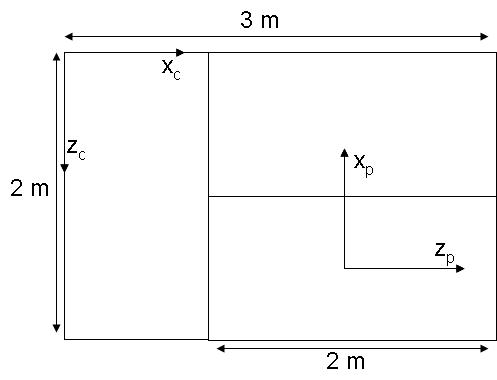
\includegraphics[height=60mm]{pics/3body_arrange.jpg}
\caption{Diagram of Reattached Body}
\label{3body_arrange}
\end{center}
\end{figure}



\item[Results:]\ \newline
The position of the new center of mass should be up and to the left of the 
center of the parent plate, at a location $(\frac{1}{2},~0,~-\frac{1}{2})~m$ 
relative to its structure-point.

The inertia tensor of the new composite plate should be that of a rectangular 
plate of dimensions $(2,~0,~3)~m$ and mass of $3~kg$.  
\begin{equation*}
I_{parent-comp,body} = 
   \begin{bmatrix} \frac{9}{4} & 0   & 0  \\
                   0   & \frac{13}{4} & 0   \\
                    0  & 0   & 1  
   \end{bmatrix}
\end{equation*}

Since neither \textit{child1} nor \textit{child2} have children, their 
composite properties should duplicate their core properties.

All results are as expected.
\end{description}






\subsection{Inertia Specification Options}
\test{Inertia Specification Option Struct}\label{test:mass_05}
\begin{description}
\item[Purpose:] \ \newline
The purpose of this test is to confirm that the \ModelDesc
can correctly compute the inertia tensor referenced to the body-axes when the 
inertia tensor is provided referenced to an axes-set aligned with the 
body-axes, but offset from the center of mass.  This test additionally 
verifies the usage of the \textit{inertia\_spec} option \textit{Struct}, 
setting the structural-axes to be aligned with, and offset from, the 
body-axes, and using these axes for specifying the inertia tensor.

SIM directory: models/dynamics/body\_action/verif/SIM\_verif\_attach\_mass\\
Run directory: RUN\_05

\item[Requirements:] \ \newline
Successful completion of this test partially satisfies
requirement~\traceref{reqt:non_centroid_calc} (aligned and offset).

\item[Procedure:]\ \newline
The object used in this test is conceptualized as a planar object, with 
dimensions $(1.0, ~0.0, ~2.0) ~m$, with the structure point in one corner, 
structure-axes and body-axes aligned, with the body-axes along the body 
principal axes, and the inertia tensor specified using the structure-axes.

Note - The specification that we are using the structural-axes is provided 
with the \textit{Struct} option selected for the \textit{inertia\_spec} 
variable.


The inertia tensor refrenced to the body-axes for such a flat plate is:
\begin{equation*}
I_{body} = 
   \begin{bmatrix} \frac{1}{3} & 0.0   & 0.0  \\
                   0.0   & \frac{5}{12} & 0.0   \\
                    0.0  & 0.0   & \frac{1}{12} 
   \end{bmatrix}
\end{equation*} 

Transposing to one corner adjusts the inertia tensor by:

\begin{equation*}
I_{struc} = 
   \begin{bmatrix} \frac{1}{3} & 0   & 0  \\
                   0   & \frac{5}{12} & 0   \\
                   0  & 0   & \frac{1}{12} 
   \end{bmatrix}
   +
   \begin{bmatrix} 1 & 0   & -\frac{1}{2}  \\
                   0   & \frac{5}{4} & 0   \\
                   -\frac{1}{2} & 0   & \frac{1}{4} 
   \end{bmatrix}
   =
   \begin{bmatrix} \frac{4}{3} & 0   & -\frac{1}{2}  \\
                   0   & \frac{5}{3} & 0   \\
                   -\frac{1}{2} & 0   & \frac{1}{3} 
   \end{bmatrix}
\end{equation*} 

Using this value as the specified inertia tensor, adding that the inertia is 
specified in the structural, and offsetting the position of the center of mass 
with respect to structural to be at $(0.5, 0.0, 1.0)~m$, the model should 
produce the correct inertia tensor about the center of mass.

\item[Results:]\ \newline
The mass, position, orientation, and inertia tensor all agree with expected 
values.
\end{description}








\test{Inertia Specification Option, StructCG}\label{test:mass_09}
\begin{description}
\item[Purpose:] \ \newline
The purpose of this test is to confirm that:
\begin{enumerate}
 \item  The \ModelDesc 
can correctly compute the inertia tensor referenced to the body-axes when the 
inertia tensor is provided referenced to an axes-set that 
has its origin at the center of mass, but is misaligned with the body-axes.
\item The inertia-tensor will be correctly computed referenced to non-principal
axes.
\item The \textit{inertia\_spec} option \textit{StructCG} functions as 
expected.  For purposes of this verification, the specified inertia tensor is 
referenced to the structural-axes, which are set to 
be co-located with, but rotated with respect 
to, the body-axes.
\item A body so defined can be used as the parent in a 
subsequent attach process.
\end{enumerate}

SIM directory: models/dynamics/body\_action/verif/SIM\_verif\_attach\_mass\\
Run directory: RUN\_09 RUN\_109


\item[Requirements:] \ \newline
Successful completion of this test partially satisfies
requirement~\traceref{reqt:non_centroid_calc} (mis-aligned and co-located).


\item[Procedure:]\ \newline
This test utilizes two objects, both flat plates similar to that used in 
test~\ref{test:mass_05}, with dimensions $(1.0, ~0.0, ~2.0) ~m$.  The two 
plates are joined edge-to-edge to 
make one uniform flat plate of dimension $(2.0, ~0.0, ~2.0) ~m$.

Following the system established in previous tests, RUN\_09 has the attachment 
performed using offset-orientation specification, while RUN\_109 uses the 
mass-point specification to perform the same task.

Both plates have a  
structure-point at the center of the plate, and structural-axes aligned with 
the principle axes of the plate.  For the child, the body-axes are aligned 
with the structural-axes, while for the parent they are rotated.

The inertia tensor - referenced to the structural-axes, and body-axes of the 
child - is that of a flat plate referenced to its principal axes, the same as 
for the body-axes from test~\ref{test:mass_05}
\begin{equation*}
I_{struc} = 
   \begin{bmatrix} \frac{1}{3} & 0.0   & 0.0  \\
                   0.0   & \frac{5}{12} & 0.0   \\
                    0.0  & 0.0   & \frac{1}{12} 
   \end{bmatrix}
\end{equation*}

For the parent, the body axes are rotated with respect to the structural axes 
such that the transformation matrix from structural to body is
$
   \begin{bmatrix} \frac{\sqrt{3}}{2} & -\frac{1}{2}   & 0  \\
                   \frac{1}{2\sqrt{2}}   & \frac{\sqrt{3}}{2\sqrt{2}} & 
                   \frac{1}{\sqrt{2}}   \\
                   -\frac{1}{2\sqrt{2}}   & -\frac{\sqrt{3}}{2\sqrt{2}} & 
                   \frac{1}{\sqrt{2}} 
   \end{bmatrix}
$

Consequently, the core-body inertia tensor (referenced to the core-body-axes) 
for the parent is
 \begin{equation}
I_{parent-core, body} = T_{struc \rightarrow body} I_{struc} T_{body 
\rightarrow struc} = 
 \begin{bmatrix} 
 \frac{17}{48} & -\frac{\sqrt{3}}{48\sqrt{2}} & \frac{\sqrt{3}}{48\sqrt{2}}  \\
 -\frac{\sqrt{3}}{48\sqrt{2}} & \frac{23}{96} & -\frac{5}{32}   \\
 \frac{\sqrt{3}}{48\sqrt{2}} & -\frac{5}{32} & \frac{23}{96} 
   \end{bmatrix}
\label{eq:body_rotation}
\end{equation}

The child is attached to the parent such that it has a $-1.0~m$ offset on the 
x-axis, and is aligned with the parent.  After attachment, the composite-body 
should be located at $(-0.5,~0.0,~0.0)~m$.  Referenced to a set of axes 
aligned with the structural-axes, and centered at the composite center of 
mass, the composite structure has an inertia tensor equal to that of a square 
plate of side $2.0~m$ and mass $2.0~kg$
\begin{equation*}
  I_{comp,struc} = 
   \begin{bmatrix} \frac{2}{3} & 0.0   & 0.0  \\
                   0.0   & \frac{4}{3} & 0.0   \\
                    0.0  & 0.0   & \frac{2}{3} 
   \end{bmatrix}
\end{equation*}

Since the composite-body axes are aligned with the core-body axes, the same 
transformation used in equation~\ref{eq:body_rotation} must be applied to 
obtain
 \begin{equation*}
I_{composite, body} = T_{struc \rightarrow body} I_{struc} T_{body \rightarrow 
struc} = 
 \begin{bmatrix} 
 \frac{5}{6} & -\frac{1}{2\sqrt{6}} & \frac{1}{2\sqrt{6}}  \\
 -\frac{1}{2\sqrt{6}} & \frac{11}{12} & -\frac{1}{4}   \\
 \frac{1}{2\sqrt{6}} & -\frac{1}{4} & \frac{11}{12} 
   \end{bmatrix}
\end{equation*}

\item[Results:]\ \newline
The results for position and for the inertia tensors for both the core and 
composite bodies agree with predicted values.

\end{description}






\test{Inertia Specification Option SpecCG}\label{test:mass_07}
\begin{description}
\item[Purpose:] \ \newline
The purpose of this test is to exercise the usage of the 
\textit{inertia\_spec} option \textit{SpecCG}.  As with 
test~\ref{test:mass_09}, the specified inertia tensor will be referenced to an 
axes-set that 
has its origin at the center of mass, but is misaligned with the body-axes. 
For this test, neither the body-axes nor structural-axes will be used as the 
reference axes-set for the inertia-tensor; a third axes-set, the 
specified-axes, must be defined instead.
This test 
additionally confirms that a body so defined can be correctly used as the 
child in a subsequent attach process.

SIM directory: models/dynamics/body\_action/verif/SIM\_verif\_attach\_mass\\
Run directory: RUN\_07 RUN\_107


\item[Requirements:] \ \newline
Successful completion of this test partially satisfies
requirement~\traceref{reqt:non_centroid_calc} (mis-aligned and co-located, 
body-independent axes).


\item[Procedure:]\ \newline
The conceptual object used in this test comprises two identical uniform flat 
plates similar to those used in tests~\ref{test:mass_05} 
and~\ref{test:mass_09}, each with dimension $(~1.0, ~0.0, ~2.0) ~m$.  The 
child plate is attached to the parent with a $1.0~m$ offset on the x-axis, 
making an edge-to-edge attachment to form one 
uniform flat plate of dimension $(2.0, ~0.0, ~2.0) ~m$.

Following the system established in previous tests, RUN\_07 has the attachment 
performed using offset-orientation specification, while RUN\_107 uses the 
mass-point specification to perform the same task.

The parent body has body-axes and structural-axes equivalent and aligned 
with the principal axes of the plate; while the inertia tensor reference 
option (\textit{inertia\_spec} is technically \textit{StructCG}, this is 
equivalent to the body-axes anyway.  Therefore, its inertia tensor 
specified about its body axes is, as in previous tests,

\begin{equation*}
I_{Body} = 
   \begin{bmatrix} \frac{1}{3} & 0   & 0  \\
                   0   & \frac{5}{12} & 0  \\
                    0  & 0  & \frac{1}{12} 
   \end{bmatrix}
\end{equation*} 

The child body also has body-axes and structural-axes equivalent and aligned 
with the principal axes of the plate.  however, it has its inertia tensor 
specified about a set of axes located at 
the center of mass, and oriented with transformation 
matrix 
$\begin{bmatrix} \frac{\sqrt{3}}{2} & -\frac{1}{2}   & 0  \\
                   \frac{1}{2}   & \frac{\sqrt{3}}{2} & 0   \\
                    0  & 0   & 1 
   \end{bmatrix}
$
(i.e. a 30-degree rotation about the z-axis)

Note 1 - specified values are expressed with respect to structural-axes that 
are aligned with body-axes  

Note 2 - The specification that we are using an oriented axes-set with origin 
at the center of mass is provided with the \textit{SpecCG} option selected for 
the \textit{inertia\_spec} variable.

The effective inertia tensor referenced to these axes can be found thus:
\begin{equation*}
I_{oriented-axes} = T_{body \rightarrow orient} I_{body} T_{orient \rightarrow 
body} = 
   \begin{bmatrix} \frac{17}{48} & \frac{\sqrt{3}}{48}   & 0  \\
                   \frac{\sqrt{3}}{48}   & \frac{19}{48} & 0   \\
                    0  & 0  & \frac{1}{12} 
   \end{bmatrix}
\end{equation*}

\item[Results:]\ \newline
With the inputs provided, the composite-body should have position at $(0.5, 
~0.0, ~0.0)~m$ and an inertia tensor equal to that of a flat square plate of 
mass $2.0 ~kg$ and side $2.0 ~m$.:

\begin{equation*}
I_{composite, body} = 
   \begin{bmatrix} \frac{2}{3} & 0 & 0  \\
                   0   & \frac{4}{3} & 0   \\
                    0  & 0  & \frac{2}{3} 
   \end{bmatrix}
\end{equation*}

The output from the test matches the analytic prediction.
\end{description}
















\test{Inertia Specification Option Spec}\label{test:mass_06}
\begin{description}
\item[Purpose:] \ \newline
The purpose of this test is to build upon the results of 
test~\ref{test:mass_05} and test~\ref{test:mass_07} to confirm that the 
\ModelDesc can correctly compute the inertia tensor referenced to the 
body-axes 
when the inertia tensor is provided referenced to an axes-set that is both 
mis-aligned with the 
body-axes, and offset from the center of mass.  As with 
test~\ref{test:mass_07}, this test 
additionally confirms that a body so defined can be correctly attached to 
another body.

SIM directory: models/dynamics/body\_action/verif/SIM\_verif\_attach\_mass\\
Run directory: RUN\_06 RUN\_106


\item[Requirements:] \ \newline
Successful completion of this test partially satisfies
requirement~\traceref{reqt:non_centroid_calc} (mis-aligned and offset, 
body-independent axes).


\item[Procedure:]\ \newline
The conceptual object used in this test comprises two identical uniform flat 
plates with dimension $(~1.0, ~0.0, ~2.0) ~m$, joined end-to-end to make one 
uniform flat plate of dimension $(1.0, ~0.0, ~4.0) ~m$.

Following the system established in previous tests, RUN\_06 has the attachment 
performed using offset-orientation specification, while RUN\_106 uses the 
mass-point specification to perform the same task.

The parent body has its inertia tensor referenced to its body axes
\begin{equation*}
I_{core, body} = 
   \begin{bmatrix} \frac{1}{3} & 0   & 0  \\
                   0   & \frac{5}{12} & 0   \\
                    0  & 0   & \frac{1}{12} 
   \end{bmatrix}
\end{equation*} 

The child body has its inertia tensor referenced to a set of axes located at 
$(\frac{\sqrt{3}}{4}, ~-\frac{1}{4}, ~1)~m$, and oriented with transformation 
matrix 
$\begin{bmatrix} \frac{\sqrt{3}}{2} & -\frac{1}{2}   & 0  \\
                   \frac{1}{2}   & \frac{\sqrt{3}}{2} & 0  \\
                    0  & 0   & 1 
   \end{bmatrix}
$
(i.e. a 30-degree rotation about the z-axis)

Note 1 - specified values are expressed with respect to structural-axes that 
are aligned with body-axes  

Note 2 - The specification that we are using an oriented axes-set with offset 
origin is provided with the \textit{Spec} option selected for the 
\textit{inertia\_spec} variable.
 
 The effective inertia tensor referenced to these axes is:
 \begin{equation*}
I_{core, specified-axes} = 
   \begin{bmatrix} \frac{5}{12} & \frac{\sqrt{3}}{12}   & -\frac{\sqrt{3}}{4}  
   \\
                   \frac{\sqrt{3}}{12}   & \frac{19}{12} & \frac{1}{4}   \\
                    -\frac{\sqrt{3}}{4}  & \frac{1}{4}   & \frac{4}{3} 
   \end{bmatrix}
\end{equation*}


 
\item[Results:]\ \newline
The resulting parent-based composite body should have a center of mass located 
at $(0.0,~0.0,~1.0)~m$ from the structural-point of the parent, and have an 
inertia tensor referenced to the composite-body-axes equal to that of a 
uniform rectangular plate of mass $2.0~kg$ and sides $(1.0,~0.0,~4.0)~m$.

\begin{equation*}
I_{parent-composite,body} = 
   \begin{bmatrix} \frac{8}{3} & 0   & 0  \\
                   0   & \frac{34}{12} & 0   \\
                    0  & 0   & \frac{1}{6} 
   \end{bmatrix}
\end{equation*} 

Results agree with expected values to within expected numerical precision.
\end{description}


















\subsection{Test in Simulation Environment}
\test{SIM Apollo}\label{test:mass_12}
\begin{description}
\item[Purpose:] \ \newline
The purpose of this test is to verif the attach and detach functionality of the
\ModelDesc during operation of a regular simulation.  This
is accomplished by creating a column of attached vehicles to simulate the 
prelaunch stack of 
an Apollo mission.  Then in a very short time frame the vehicles are detached 
and reattached 
as appropriate in an Apollo mission.\\
SIM directory: sims/SIM\_Apollo\\
Run directory: RUN\_test
\item[Requirements:] \ \newline
Successful completion of this test confirms that the results of the previous 
verification tests are legitimate in a simulation environment.  It partially satisfies requirements~\traceref{reqt:CoM_location}, \traceref{reqt:composite_mass}, 
\traceref{reqt:composite_inertia}, \traceref{reqt:non_centroid_calc}, 
\traceref{reqt:attach}, \traceref{reqt:detach}, and \traceref{reqt:mass_reattach}.
\item[Procedure:]\ \newline
In this Apollo simulation the Satern V launch stack detaches mass bodies in 
the samee order as a real Apollo mission, but 
in a condensed time frame (12 seconds).
\begin{enumerate}
\item{Detach the first stage.}
\item{Detach the second stage.}
\item{Detach the third stage.}
\item{Detach the LEM.}
\item{Attach LEM to CM.}
\item{Detach the LEM.}
\item{Detach the LEM descent stage.}
\item{Attach LEM to CM.}
\item{Detach the LEM for last time.}
\end{enumerate}
\item[Results:]\ \newline
The \ModelDesc\ utilization in SIM\_Apollo successfully demonstrates run-time 
attach and detach operations.
\end{description}

%\section{Requirements Traceability}\label{sec:traceability}
\begin{table}[ht]\label{tab:reqt_ivv_xref}
\begin{tabular}{||p{3.2in}|p{3.2in}|} \hline
{\bf Requirement} & {\bf Inspection or test} \\ \hline \hline
\ref{reqt:jeod} - Top-level requirements &
  Insp. \ref{inspect:jeod} - meets Top-level \\ \hline
\ref{reqt:CoM_location} - Center of Mass Location &
  All tests  \\ \hline
\ref{reqt:composite_mass} - Composite Mass Calculation &
  All tests  \\ \hline
\ref{reqt:composite_inertia} - Composite Inertia Calculation &
  All tests  \\ \hline
\ref{reqt:attach_detach} - Attach and Detach Masses &
  Attachment: All tests \\
& Detachment: Test \ref{test:mass_12} - SIM\_Apollo \\ \hline
\ref{reqt:non_centroid_calc} - Non-centroidal Inertia Calculations &
  Test. \ref{test:mass_10} - 4 Thin Plates with Detachment \\ \hline
\ref{reqt:mass_reattach} - Reattach Child to Parent &
  Test. \ref{test:mass_12} - SIM\_Apollo \\ 
& Test. \ref{test:mass_10} - 4 Thin Plates with Detachment \\ \hline
\ref{reqt:mass_extend} - Model extension &
  Insp. \ref{inspect:mass_extend} - Dynamics Body model \\ \hline
\end{tabular}
\caption{Requirements Traceability}
\end{table}